\documentclass[Report.tex]{subfiles}
\begin{document}

\chapter{Testing and Optimisation}
Unit testing and manual testing methods were employed throughout development to ensure that each function continued to return results as expected. An example of a typical unit test is outlined in this chapter, with further elaboration on the methodology employed. A large part of this project concerned the retrieval and manipulation of data from various sources. Refining the input to the APIs and databases resulted in higher success rates of the queries, the creation of more informative datasets, and improved representation of data on the client side. The process of improving these aspects was iterative, and each modification was tested to assess whether the change in output had a positive effect. The key changes in geocoding, querying the MySQL database for concepts, and ordering the concept are discussed in the current chapter.

\section{Testing}
\subsection{Unit Testing}
Unit tests were written for key functions during development. This was important as the project consists of numerous modules, each of which contributes toward the end result; if a function is modified in a way that results in an unexpected side-effect it is easier to untangle the root cause from unit tests. Many of the functions written for data manipulation involve the organisation of Python dicts and lists to fit the format expected by the external services (databases and APIs) or for parsing as JSON Objects by the client-side. Test-Driven Development was utilised for these purposes, as the outcome was known before development began and tests could then be run to determine whether the function returned results as expected. To ensure maximum efficacy of these tests, production of side effects was reduced as much as was possible. \newline

\noindent The key modules 'geocode', 'metamap', 'umls' and 'citations' each interacted with an external service, making automated testing laborious and time-consuming. In many cases it can be assumed that the service is working correctly, or any problems are beyond the scope of the application. Therefore, the functionality being tested was often not the HTTP requests and database calls themselves, but the Python underlying these calls. The Python library unittest.mock enables the patching of methods by decorating the test: the \texttt{@patch} decorator receives the function to patch as an argument, and returns the Mock object which is passed as an argument. Within the test, any calls to the patched function will behave as specified without any calls to the 'real' function. An example test has been included below, where the \texttt{geocode.request} function has been patched to return the expected output.\newline

\begin{lstlisting}
@patch('app.geocode.request')
def test_run(self, mock_request):
    # patch geocode.request with example available from API docs
    mock_request.return_value = fake_json('places_search_output.json')

    # get_location_output.json contains one result from Places API
    place_result = fake_json('get_location_output.json')

    expected = {
        'results': [
            {
                'PMID': '00000000',
                'place': place_result
            },
            {
                'PMID': '00000001',
                'place': place_result
            }
        ],
       'for_cache': [
            {
                'PMID': '00000000',
                'placeids': [
                    'ChIJyWEHuEmuEmsRm9hTkapTCrk'
                ]
            },
            {
                'PMID': '00000001',
                'placeids': [
                    'ChIJyWEHuEmuEmsRm9hTkapTCrk'
                ]
            }
        ]
    }

    observed = geocode.run(fake_json('eFetch_sample.json'))
    
    self.assertEqual(mock_request.call_count, 2)
    self.maxDiff = None
    self.assertEqual(observed, expected)
\end{lstlisting}\newpage

\subsection{Manual Testing}
Broader testing of the application was carried out manually, to assess whether the system was functioning as a whole and returning the expected results in line with the input query. Statements are printed to the console at the start and end of key processes to keep track of what stage the application is in. This is particularly useful if one of the services hangs. A log file is written to show the results of individual queries, an example of which can be seen in Appendix \ref{App:AppendixA}. 

\section{Optimisation}
\subsection{Geocoding}
The overhead of geocoding an address for the first time is high; the Text Search service in the Google Places API returns the top ten results that match the input parameters. In order to try and make the results more precise, the 'types' parameter is provided to specify that results should be either a university, a hospital, or an 'establishment' which is set as the default if a type is not present. In order to maximise the number of meaningful results achieved by the API, the input must be optimised to improve the chance that any location is returned (from this point onward referred to as the 'hit rate') and accuracy of the geocoding process. A number of formatting options were empirically tested, enabling an informed decision to be made for the geocoding function in the application.\newline

\noindent In order to have confidence in applying these findings to the larger population of papers available on PubMed, a dataset with papers on a range of topics, from various journals, and originating from numerous countries was required. Statistics on the publishing distribution between countries was found on Medline Trend\cite{medlinetrend}, though the data was limited to a date range of 2008-2012. Table \ref{tab:countries} lists the ten countries with the most papers, their percentage share and the corresponding number of papers used in the dataset. Though the intention was to have the number of addresses reflect these data, each paper in the dataset has multiple affiliation addresses, skewing the distribution. Thus, the primary feature of the dataset is that each of these countries is represented at least once. 33 unique papers and 178 addresses were included to assess the hit rate, and 10 papers and 18 addresses were included to assess the accuracy. Expected locations were found manually using the Google Maps website, and therefore were tested at a smaller scale. The distance between the 'true' location and the geographical coordinates as returned by the Places API could then be compared. A radius of 5 kilometres was chosen as the cut-off distance for a location to be called as accurate. It is important to note that the allocation of correct addresses was somewhat subjective. Automation would have been preferred, however it was not possible to retrieve papers with exclusively the affiliation address in the query. Even if this could have been achieved, universities with campuses distributed over a large area may have produced misleading conclusions.\newpage

\begin{table}
\begin{center}
    \begin{tabular}{ | l | c | c | }\hline
    \textbf{Country} & \textbf{Papers (\%)} & \textbf{Papers in} \\
     & &\textbf{dataset}\\ \hline
    USA & 28.1 & 14\\ \hline
    China & 8.5 & 4\\ \hline
    United Kingdom & 7.7 & 4\\ \hline
    Japan & 5.8 & 3\\ \hline
    Germany & 5.1 & 3\\ \hline
    Italy & 3.7 & 2\\ \hline
    Canada & 3.5 & 2\\ \hline
    France & 3.5 & 2\\ \hline
    Australia & 2.6 & 1\\ \hline
    India & 2.6 & 1\\ \hline
    \end{tabular}
    \caption{Percentage share of published papers between 2008 and 2012 for the 10 countries with the highest values.\label{tab:countries}}
\end{center}
\end{table}

\noindent A number of formatting combinations were tested, as detailed in Figure \ref{fig:geoscatter}. As expected, there was an inverse correlation between the hit rate and the accuracy of geocoding; sending more information (a higher number of address lines, particularly at the start of the address) reduces the chance of a match to a location, however the location is more likely to be correct.\newline

\begin{figure}[h!]
	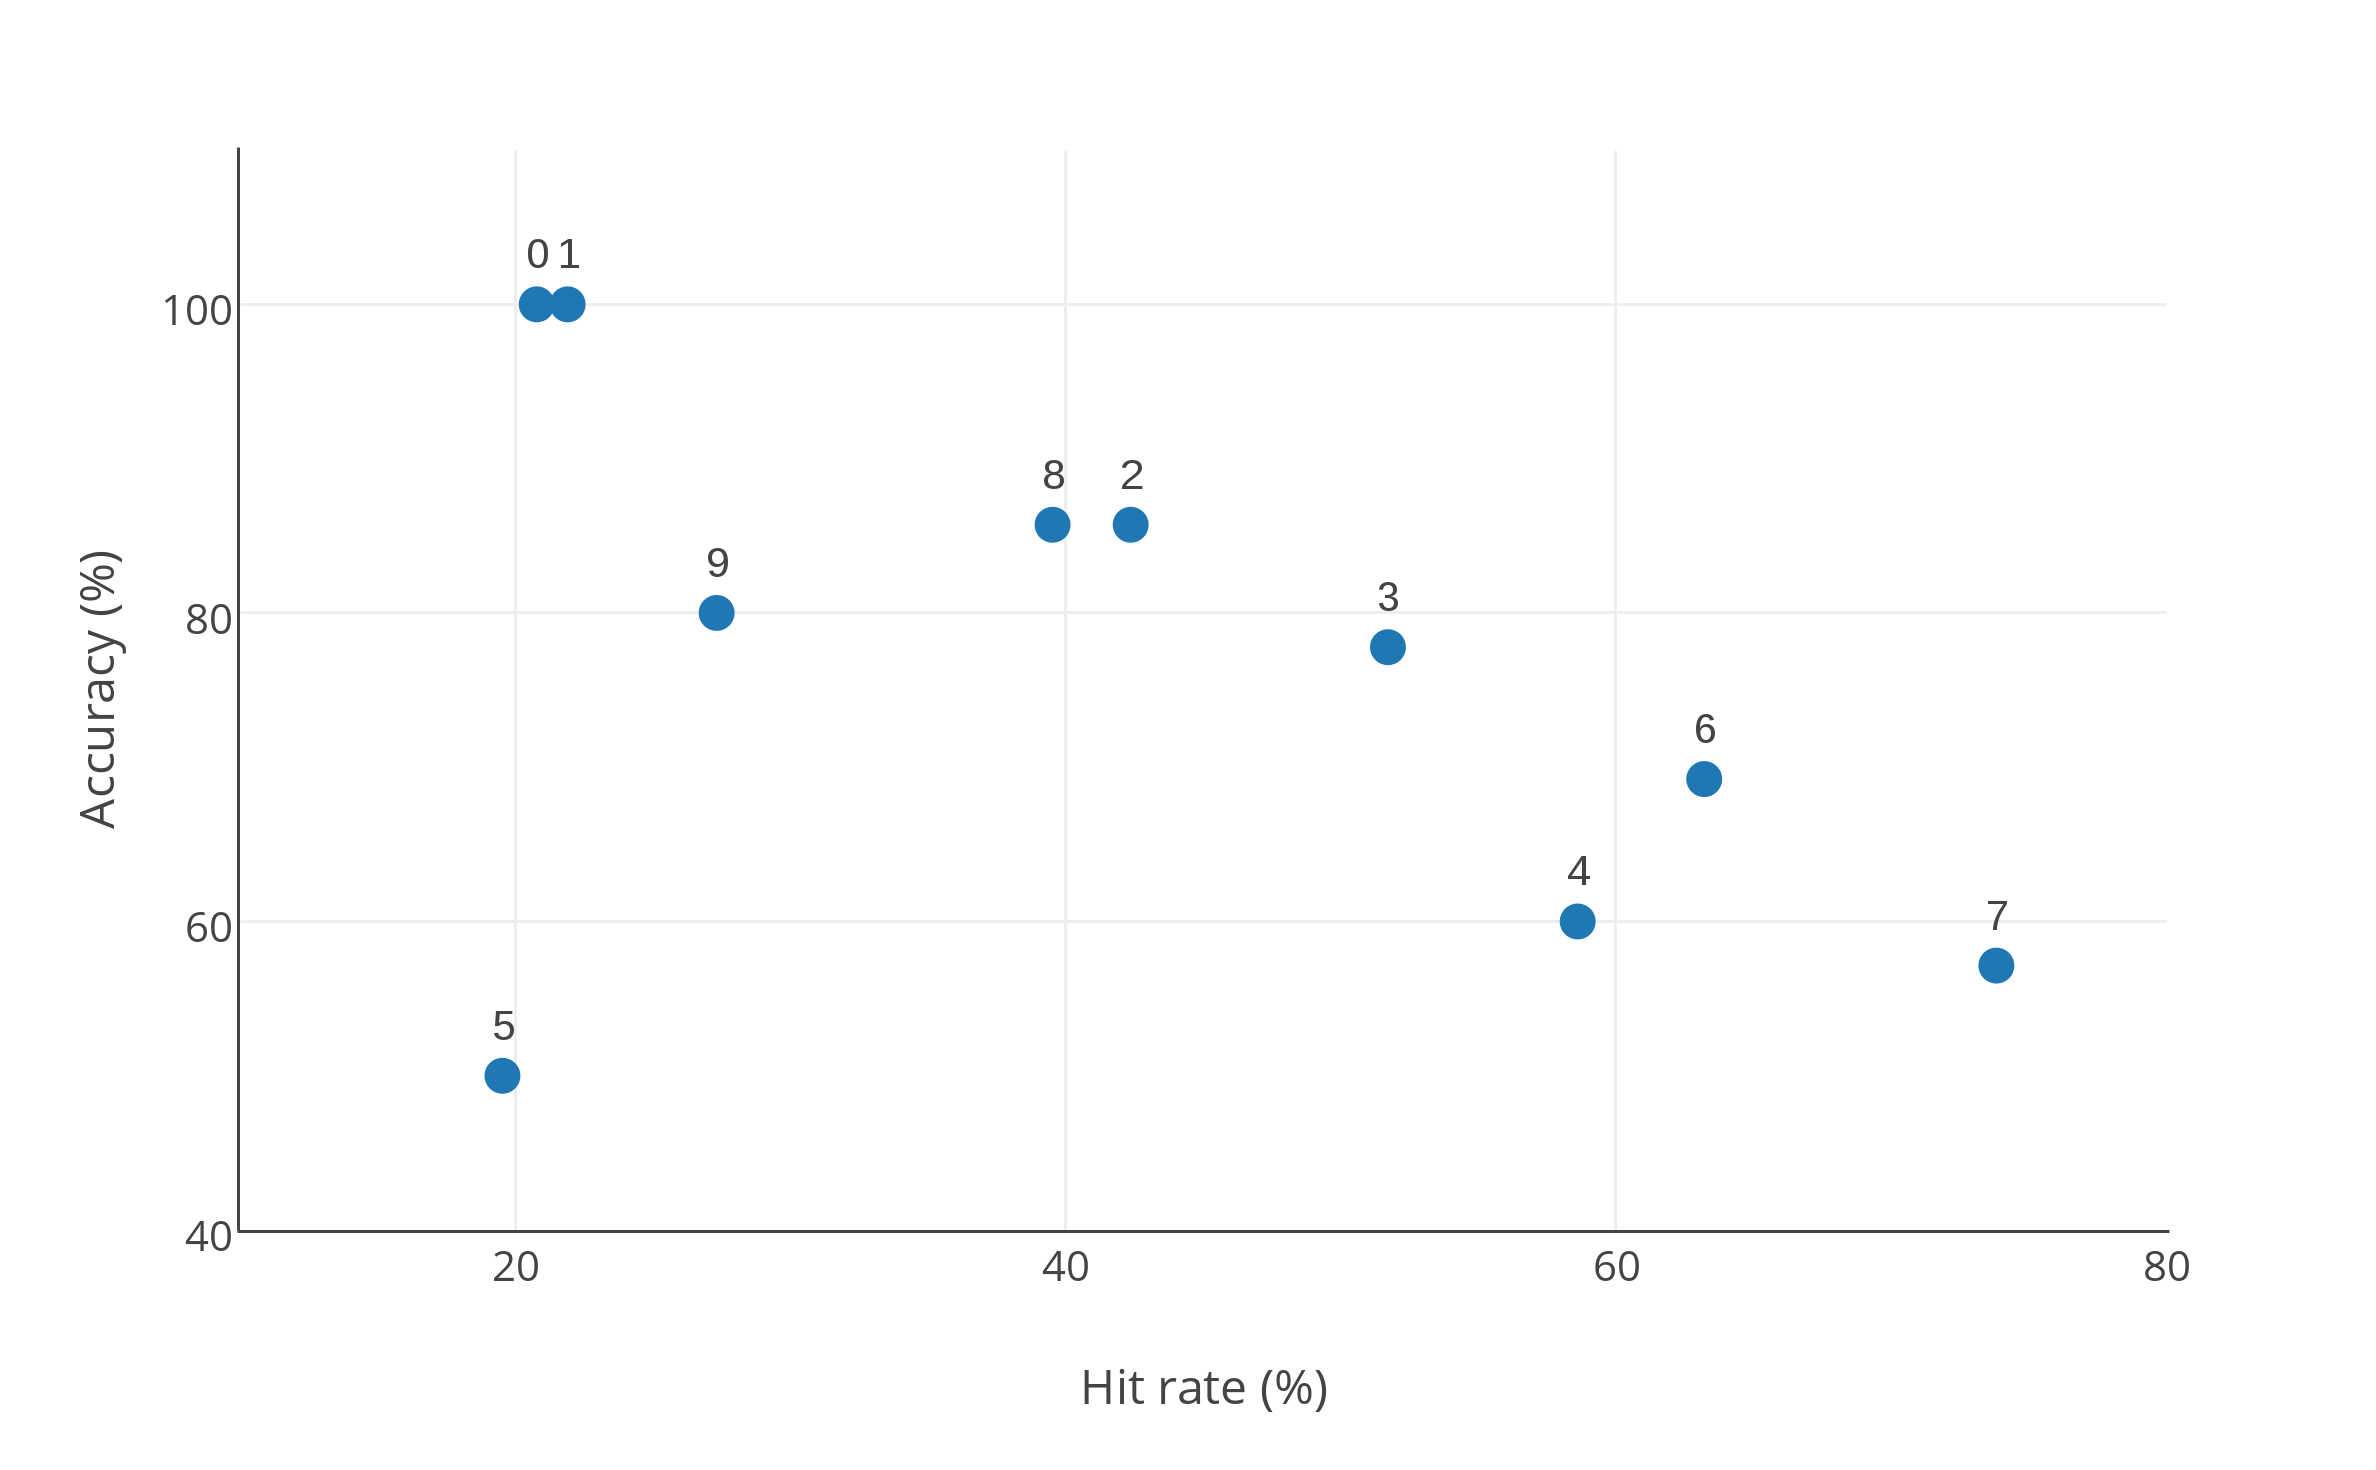
\includegraphics[width=\textwidth]{../lib/images/geocode_performance_scatter}
	\caption{The hit rate (proportion of searches that returned any result, x-axis) and accuracy (proportion of searches that returned a result within 5 km of the expected loaction, y-axis) of 10 formatting options are plotted on this graph. The numbered points represent the following formats: 0 - none, 1 - email addresses removed, 2 - department removed, 3 - first line removed, 4 - department and first line removed, 5 - last 2 lines only, 6 - second and third lines only, 7 - second and last lines only, 8 - last 3 lines only, 9 - first 2 lines removed. Only options 0 and 1 include all addresses, as they are not limited by the number of lines in an address. \label{fig:geoscatter}}
\end{figure}

\noindent The first optimisations were carried out after observing trends during development. Email addresses of the lead author are sometimes included at the end of their affiliation address, which appeared to obfuscate the address for the Google Places API. Regular expressions were implemented from the 're' Python module in order to remove strings that matched the expected pattern for emails. As can be seen in Figure \ref{fig:geoscatter} (points 0 \& 1), removing email addresses did improve the hit rate of geocoding by 1\%. Of 15 addresses that contained email addresses, one (the Chinese Academy of Agricultural Sciences in Beijing) was matched to a location before removal of the email address. After formatting to remove the email address, 3 additional addresses were successfully matched to a location, however the Beijing address could not be matched. By checking the coordinates of the original returned address, it appears that the geocoding algorithm incorporated the email string to match the address to the Natural History Museum in London. In the accuracy dataset, 3 addresses included an email address but the hit rate was zero both before and after removal of the email address. From the incongruous result seen in the hit rate data, a tentative conclusion can be drawn that removing the email address improves the accuracy of results, though by a nominal amount. Spurious data was also seen elsewhere in the dataset, indicating that the input query can only be optimised to a certain degree.\newpage

\noindent Removing lines with 'department' or 'dept' was compared to an uninformed removal of the first line, and then the two approaches were combined (Figure \ref{fig:geoscatter}, points 2, 3 \& 4 respectively). Removing the first line gave the best compromise between a reduced hit rate but increased accuracy, so this approach was adopted in later approaches. Sending the last two lines of each address (Figure \ref{fig:geoscatter}, point 5) resulted in a low hit rate and low accuracy results, most likely due to the number of lines averaging around 4 (Figure \ref{fig:addresslines}), resulting in addresses that only specify the region and the country. It was surprising to see that the Places API would not geocode areas such as 'TN, USA', perhaps to focus on matching addresses as the primary use case of the service.\newline

\begin{figure}[h!]
	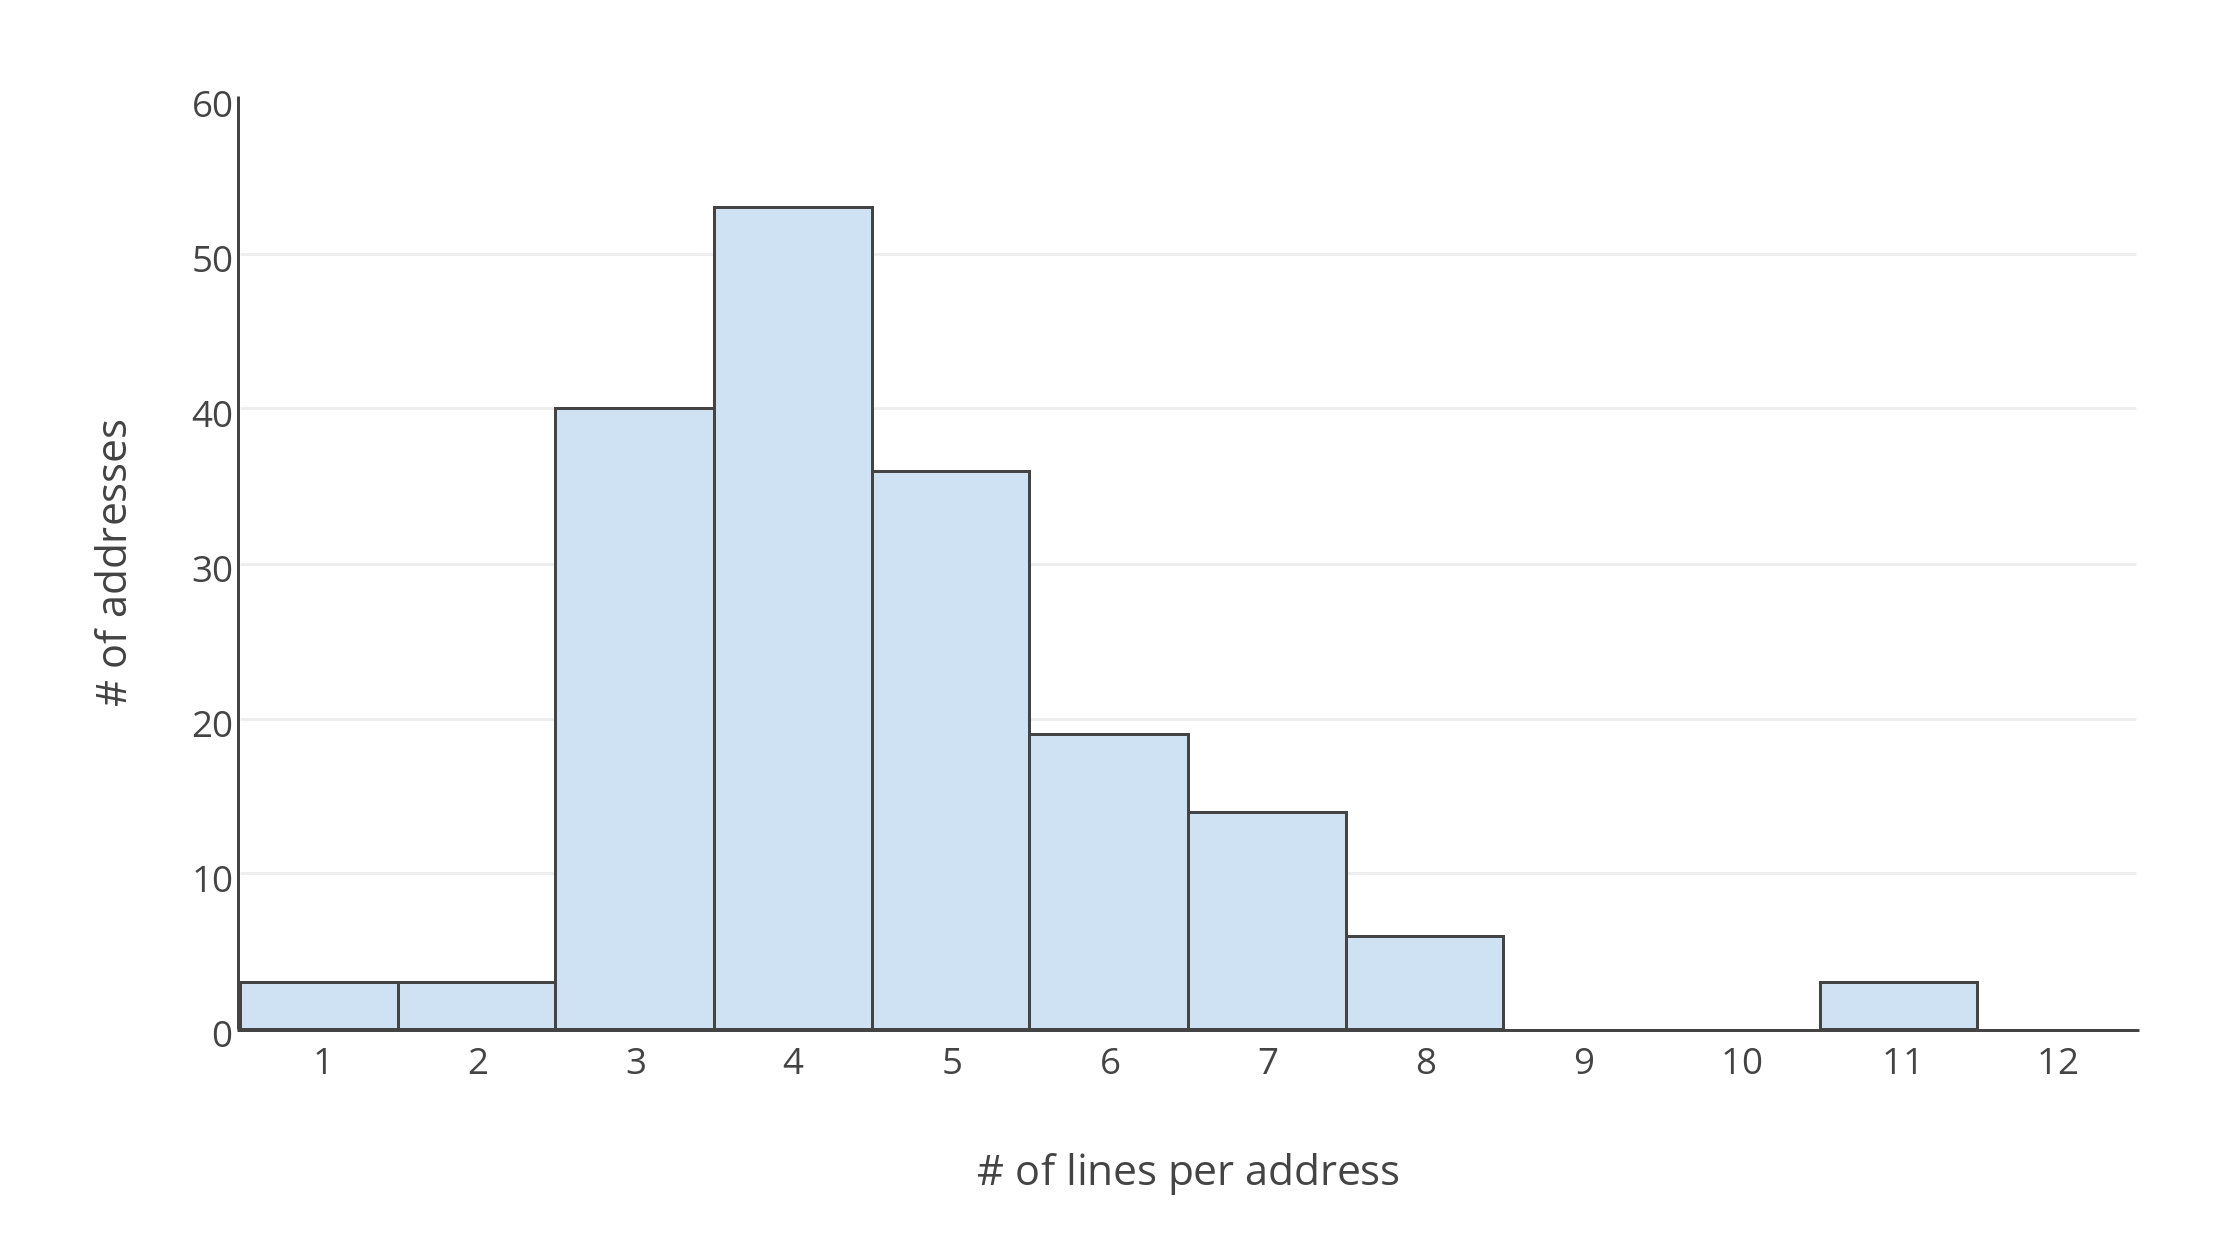
\includegraphics[width=\textwidth]{../lib/images/address-lines-histogram}
	\caption{A histogram of the number of lines found in 178 addresses.\label{fig:addresslines}}
\end{figure}

\noindent After taking into account the data in Figure \ref{fig:geoscatter}, it could be seen that there would be a trade-off between hit rate and accuracy. For the three best-performing formats, 'no department', 'no first line' and 'second and third lines' (points 2, 3 \& 6, respectively), the distances were plotted to see the distribution of data (Figure \ref{fig:geoboxes}). With each limiting formatting change from left to right, the dataset is expanded to include outliers of increasing frequency and inaccuracy. For example, the outlier 23 km away occurs in an address with the first line removed because the Places API returns the coordinates for an alternative campus. This type of inaccuracy, though sub-optimal, is permissible for this pilot version of the project. In contrast, an outlier 1336 km away occurs when only the second and third lines are used in one address; this kind of data is highly unrepresentative of the input data. These data informed the decision to format all addresses to exclude the first line and any email addresses.

\begin{figure}[h!]
	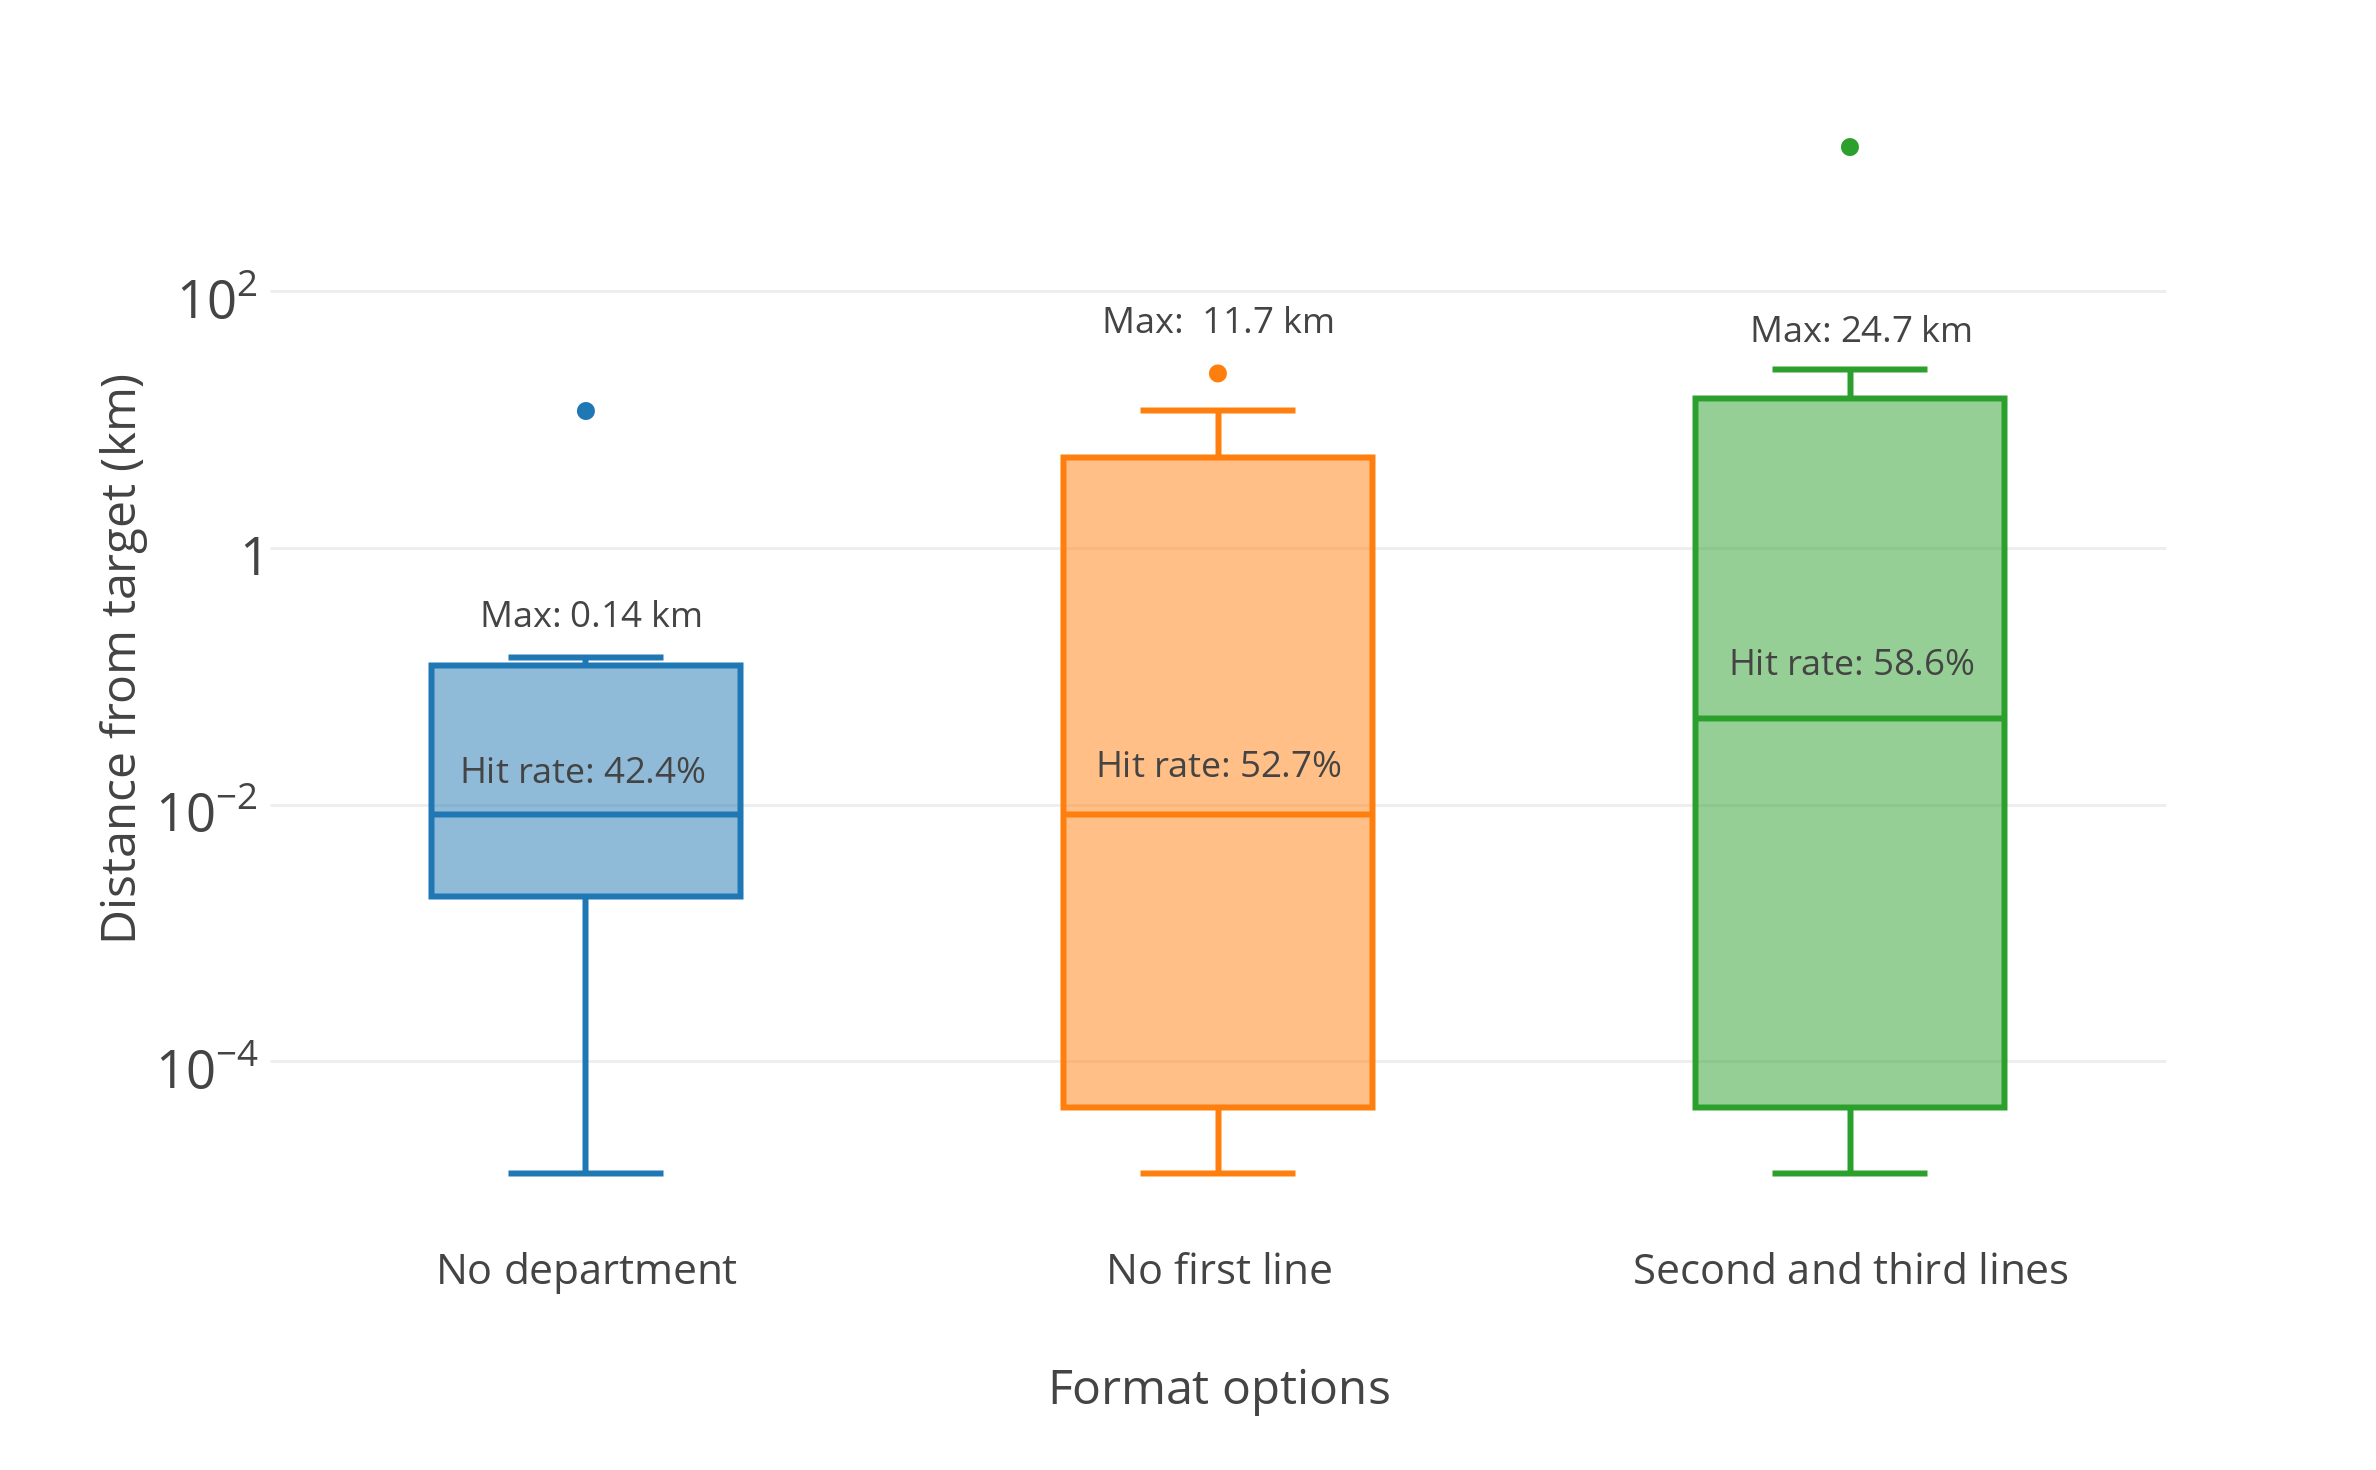
\includegraphics[width=\textwidth]{../lib/images/distance-boxes}
	\caption{Box and Whisker diagrams for 3 formats with balanced hit rates and accuracies. Key values have been added to the diagram to allow clearer comparison, as the y-axis is log10 scale.\label{fig:geoboxes}}
\end{figure}

\subsection{Querying MySQL for concept hierarchies}
Several 

\subsection{Organising Hierarchical Data}

\end{document}